\documentclass[a4paper,12pt]{article}
\usepackage[a4paper, margin=1in]{geometry}


\usepackage{etoolbox}  % For patching commands
% Insert a page break before every \subsection
\pretocmd{\subsection}{\clearpage}{}{}
% Insert a page break before every \subsubsection
\pretocmd{\subsubsection}{\clearpage}{}{}

\usepackage{ltablex}
\keepXColumns
\setcounter{tocdepth}{3}
\usepackage{array}
\newcolumntype{L}[1]{>{\raggedright\arraybackslash}p{#1}}
\usepackage{amsmath}
\usepackage{fancyhdr}
\usepackage{graphicx}
\usepackage{hyperref}
\usepackage{titlesec}
\usepackage{tabularx}
\usepackage{tocloft}
\usepackage{footnote}
\usepackage{float}
\usepackage{booktabs}
\usepackage{longtable}
\usepackage{mathptmx}
\usepackage{ragged2e}
\usepackage{longtable}
\usepackage{threeparttablex}
\makesavenoteenv{tabular}
\makesavenoteenv{table}
\renewcommand{\cftsecleader}{\cftdotfill{\cftnodots}}
\hyphenpenalty=10000
\tolerance=1000

\pagestyle{fancy}
\fancyhf{}
\fancyfoot[L]{Alfie Corthine — Candidate: T17}
\fancyfoot[C]{\thepage}

\title{\textbf{OCR A-Level Computer Science NEA} \\[0.5em] \large AI Flashcards App for iOS}
\author{Alfred Corthine}
\date{\vspace{-5ex}}

\begin{document}

\maketitle
\thispagestyle{empty}
\newpage

\tableofcontents
\newpage

\section{Analysis}

\subsection{Introduction to the Problem}
As a Sixth Form student revising for my A-Level exams, I’ve personally experienced how difficult it is to find a truly efficient and engaging method of revising large volumes of content. I often found myself copying notes back and forth or trying various study apps that promised to improve memory retention but rarely delivered. Most lacked either flexibility, intelligent feedback, or the ability to integrate with the types of notes I actually use, like PDF handouts or typed summaries. The idea for this project was born out of my own frustration and a genuine need for a smarter solution.\\

The problem I aim to solve is how to help students revise more effectively by converting their existing notes into smart flashcards and providing interactive, adaptive study tools, all within a seamless and elegant iOS app. Unlike traditional flashcard apps, mine will incorporate AI to dynamically generate questions from documents, use spaced repetition algorithms, and even offer audio-based revision via mini podcasts. This not only makes revision more effective, but also more accessible, whether a student is revising on the bus, walking home, or stuck in a queue.

\subsection{Why This Problem is Solvable Computationally}
This problem is highly amenable to computational methods because it involves repetitive data processing, structured information handling, and user-personalised feedback loops, all of which are tasks that computers excel at. Computational approaches offer scalability, consistency, and the ability to integrate intelligent automation across the entire study workflow.\\

For instance, natural language processing (NLP) algorithms can be employed to parse and understand the semantic structure of uploaded notes, textbooks, or web content. These algorithms can identify key definitions, concepts, and question-answer pairs, which can then be automatically converted into flashcards. This removes the need for users to manually create decks, a time-consuming process, while also improving consistency in formatting and content quality.\\

Databases can efficiently store, organise, and manage large volumes of flashcards, user accounts, and learning sessions. This ensures that user progress is tracked accurately over time, and that study material can be retrieved instantly across devices. Backend systems can handle multiple concurrent users and scale with demand, something manual systems cannot achieve.\\

Spaced repetition algorithms, such as those based on SuperMemo’s SM2 or more modern adaptive techniques, rely on real-time data about user performance. These algorithms can calculate optimal intervals for reviewing information, dynamically adjusting based on how well the user remembers each card. Implementing such logic computationally enables truly personalised learning experiences, something infeasible to deliver manually at scale.\\
\newpage
Additionally, computational methods make it possible to integrate features like text-to-speech, AI-generated summaries, and auto-created podcasts, allowing users to engage with content in multiple formats. These techniques rely on large language models (LLMs), machine learning, and media generation tools, all of which are built on programmable, scalable systems.\\

Finally, the problem itself is defined and constrained in a way that suits computational modelling. Inputs (e.g. notes, user answers) are structured or semi-structured, and the desired outputs (e.g. flashcards, study reminders) follow predictable patterns. This makes it feasible to encode the logic as software that can process inputs, make decisions, and generate outputs autonomously.\\

\subsection{Stakeholder Analysis}

\subsubsection*{Primary Stakeholder: Chris Chan}
Chris Chan is a Year 13 student preparing for his A-Level's. He is highly motivated but struggles with organising his revision efficiently. Chris relies on a mix of handwritten notes and PDFs from teachers, and often uses his iPhone to study on the go. His main goal is to maximise retention without spending hours rewriting notes or creating flashcards manually. Chris will use the AI Flashcards app to automatically convert his PDF/Word notes into flashcards, track his learning through spaced repetition, and revise via short audio summaries while commuting.

\subsubsection*{Secondary Stakeholder: Dr. Alice Morton}
Dr. Alice Morton, a Computer Science lecturer who works closely with sixth-form outreach programmes, regularly recommends digital tools to help students improve their independent learning. She is especially interested in how artificial intelligence can support spaced repetition and knowledge retention. Her perspective helps ensure the app remains grounded in evidence-based learning principles and is suitable for academic endorsement.

\subsubsection*{Tertiary Stakeholder: Mr. Simon Webb}
Mr. Simon Webb, a parent of two teenagers studying for their GCSEs and A-Levels, is invested in ensuring his children use mobile technology productively. While he doesn’t use the app directly, he represents the wider group of parents who value tools that encourage consistent revision habits and help reduce passive screen time. Feedback from users like Simon informs design decisions that promote healthy and educational smartphone use. \\
\newline
These stakeholders will use the app to either support their own learning (Chris), enhance their students' outcomes (Alice), or evaluate effectiveness (Simon). The design prioritises ease-of-use, accessibility, and focused content delivery.

\newpage

\subsection{Analysis of Existing Solutions}

\subsubsection{\underline{Anki}}

Anki is a highly popular, open-source flashcard application that has gained widespread acclaim in educational and professional communities for its robust and scientifically validated approach to spaced repetition. At its core, Anki employs an advanced algorithm based on the SM-2 spaced repetition system, originally developed for language learning, which schedules flashcard reviews at optimally spaced intervals to maximise long-term retention and minimise forgetting. This evidence-based approach is backed by extensive cognitive science research on memory and learning. \\

One of Anki’s standout features is its exceptional customisability. Users can create highly personalised decks with support for rich text formatting, images, audio, video, and even custom card templates using HTML and CSS. This flexibility allows learners to tailor flashcards precisely to their needs, whether they’re studying languages, medical terminology, engineering concepts, or historical facts. Furthermore, Anki supports extensive add-ons created by a passionate community, which can enhance functionality ranging from user interface improvements to detailed progress analytics and new learning modes. \\

Anki is available on multiple platforms including Windows, macOS, Linux, iOS, and Android, allowing users to synchronise their progress seamlessly across devices. Its open-source nature means that it is continuously improved by contributors globally, ensuring a vibrant ecosystem that keeps pace with emerging learning technologies and user feedback. \\

Despite its many strengths, Anki has a somewhat steep learning curve, particularly for new users who may find its interface and numerous settings overwhelming. However, this complexity is often outweighed by the power it offers dedicated learners who want to optimise their study routines and engage deeply with their materials. \\

\begin{figure}[H]
    \centering
    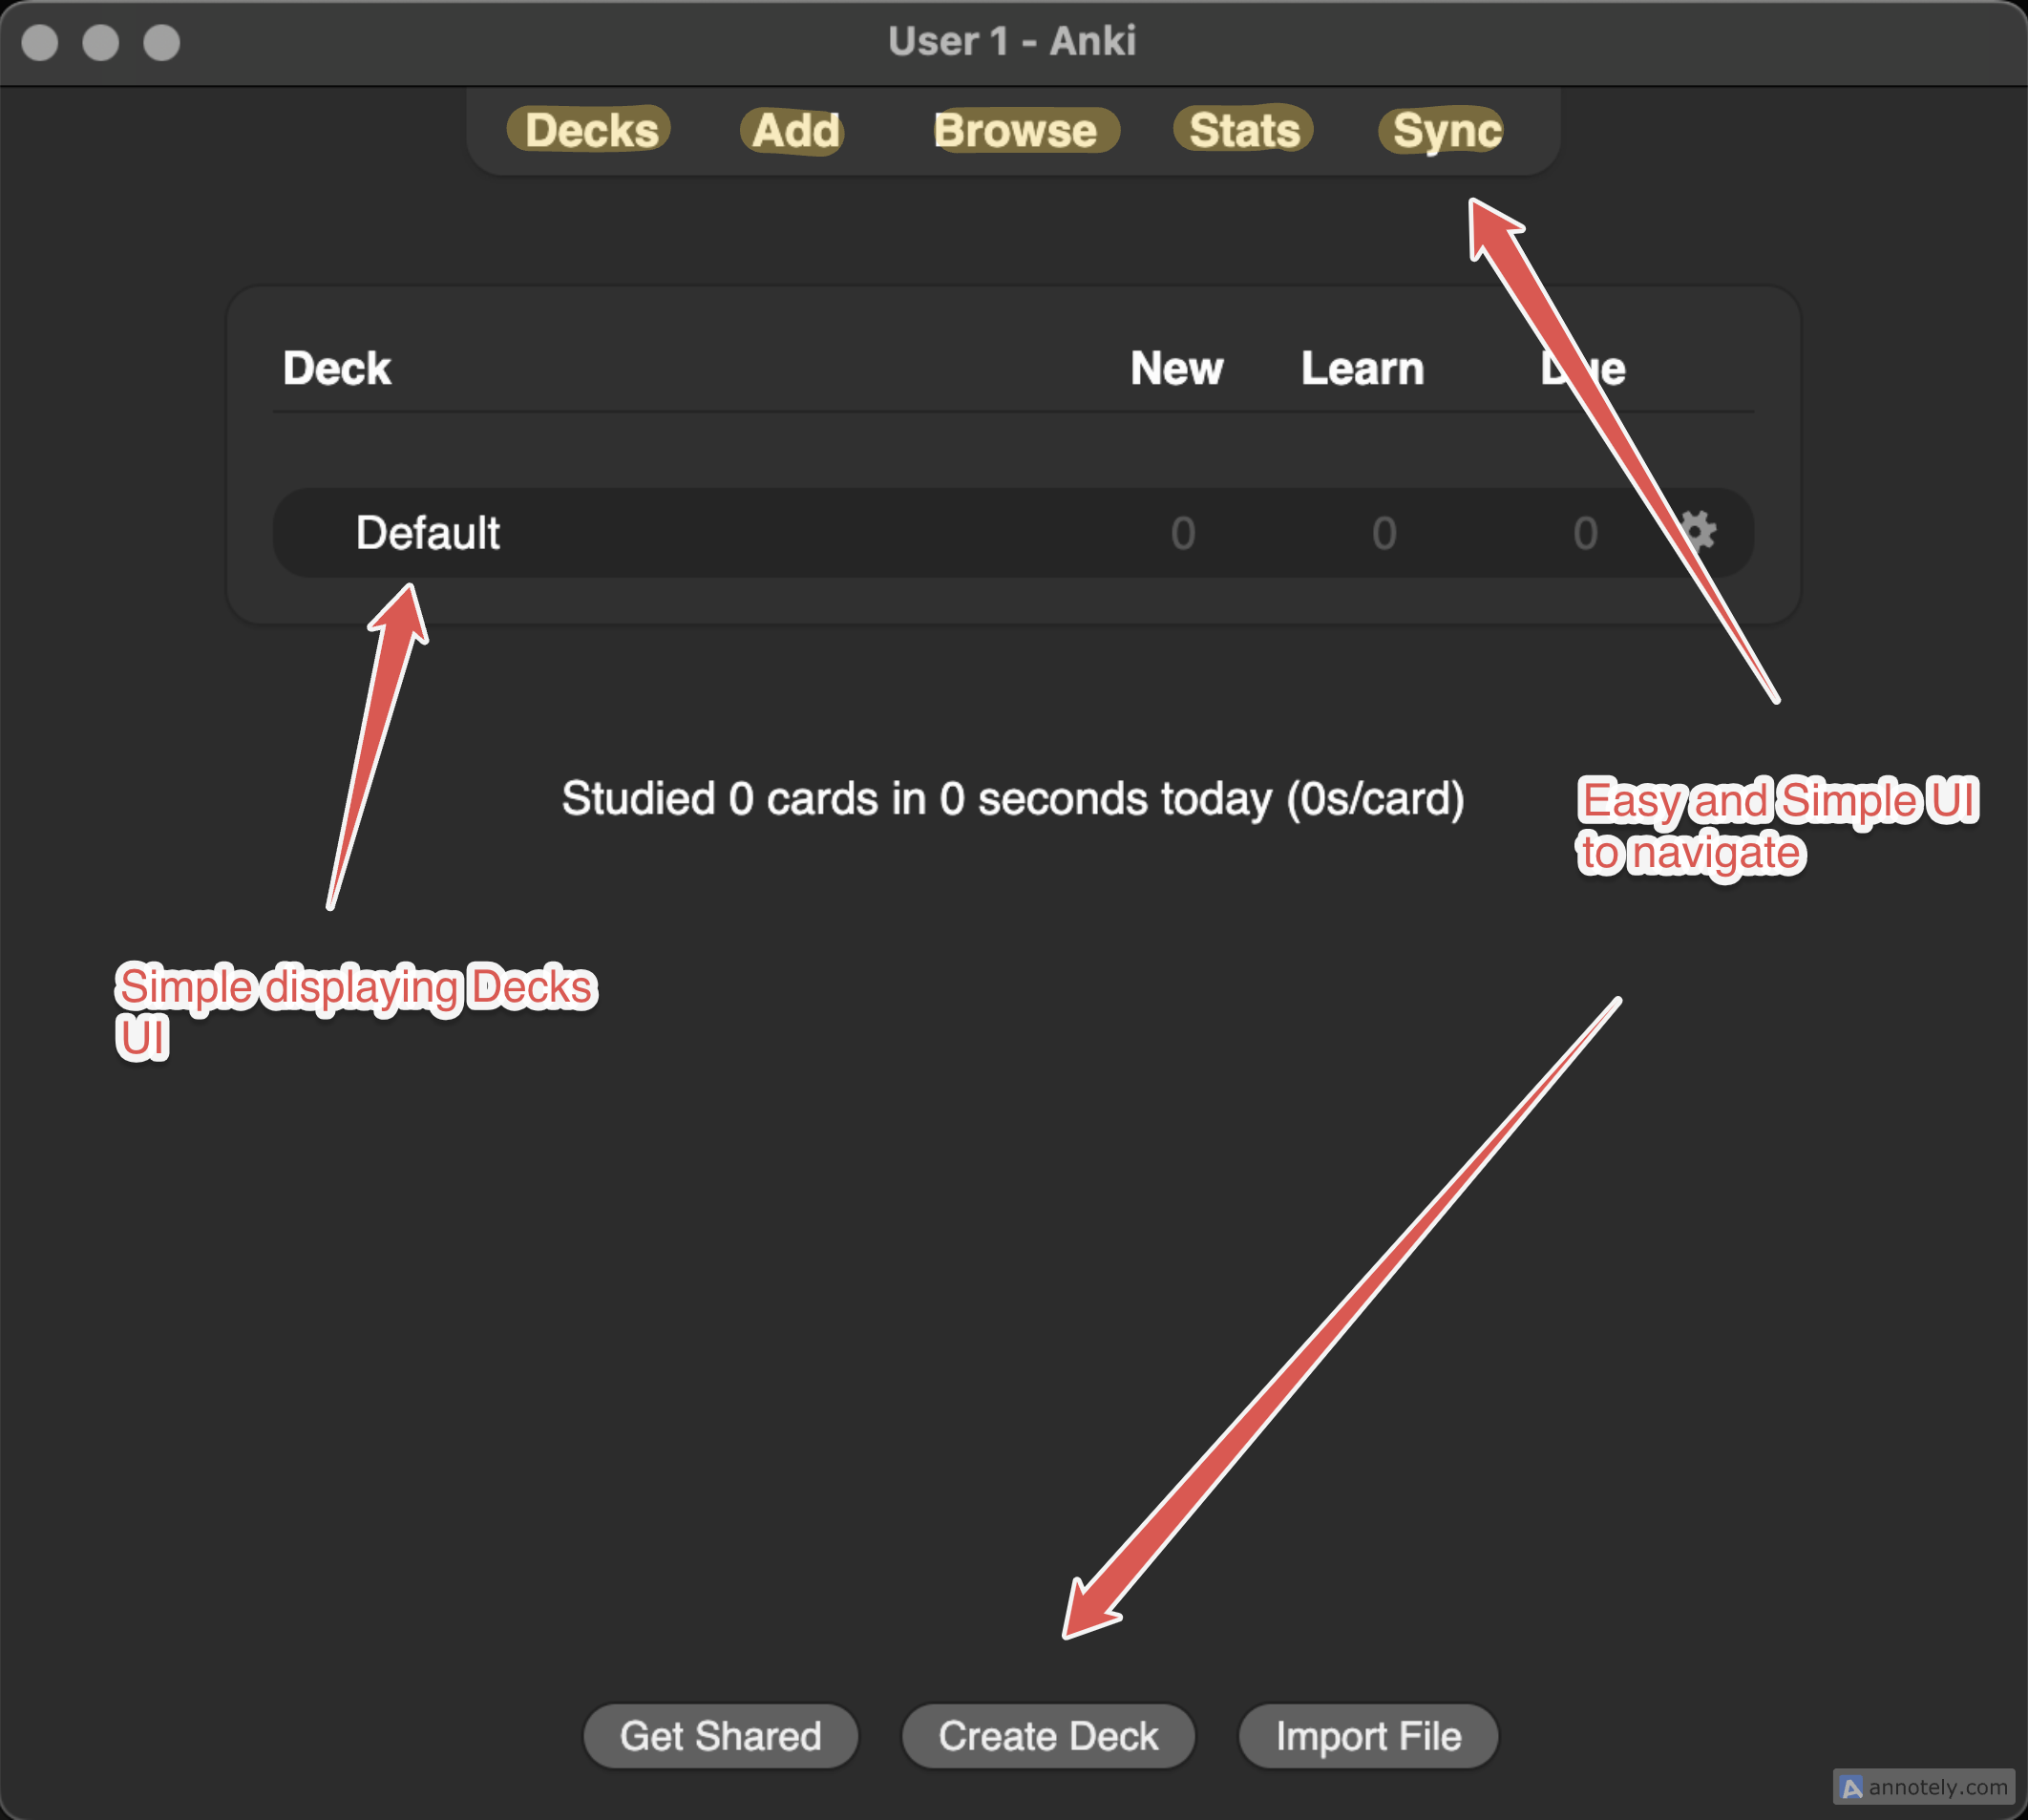
\includegraphics[width=0.7\linewidth]{../Screenshots/AnkiHome.png}
    \caption{Anki Home Menu — shows the deck list and overall navigation}
    \label{fig:anki-home}
\end{figure}

\begin{figure}[H]
    \centering
    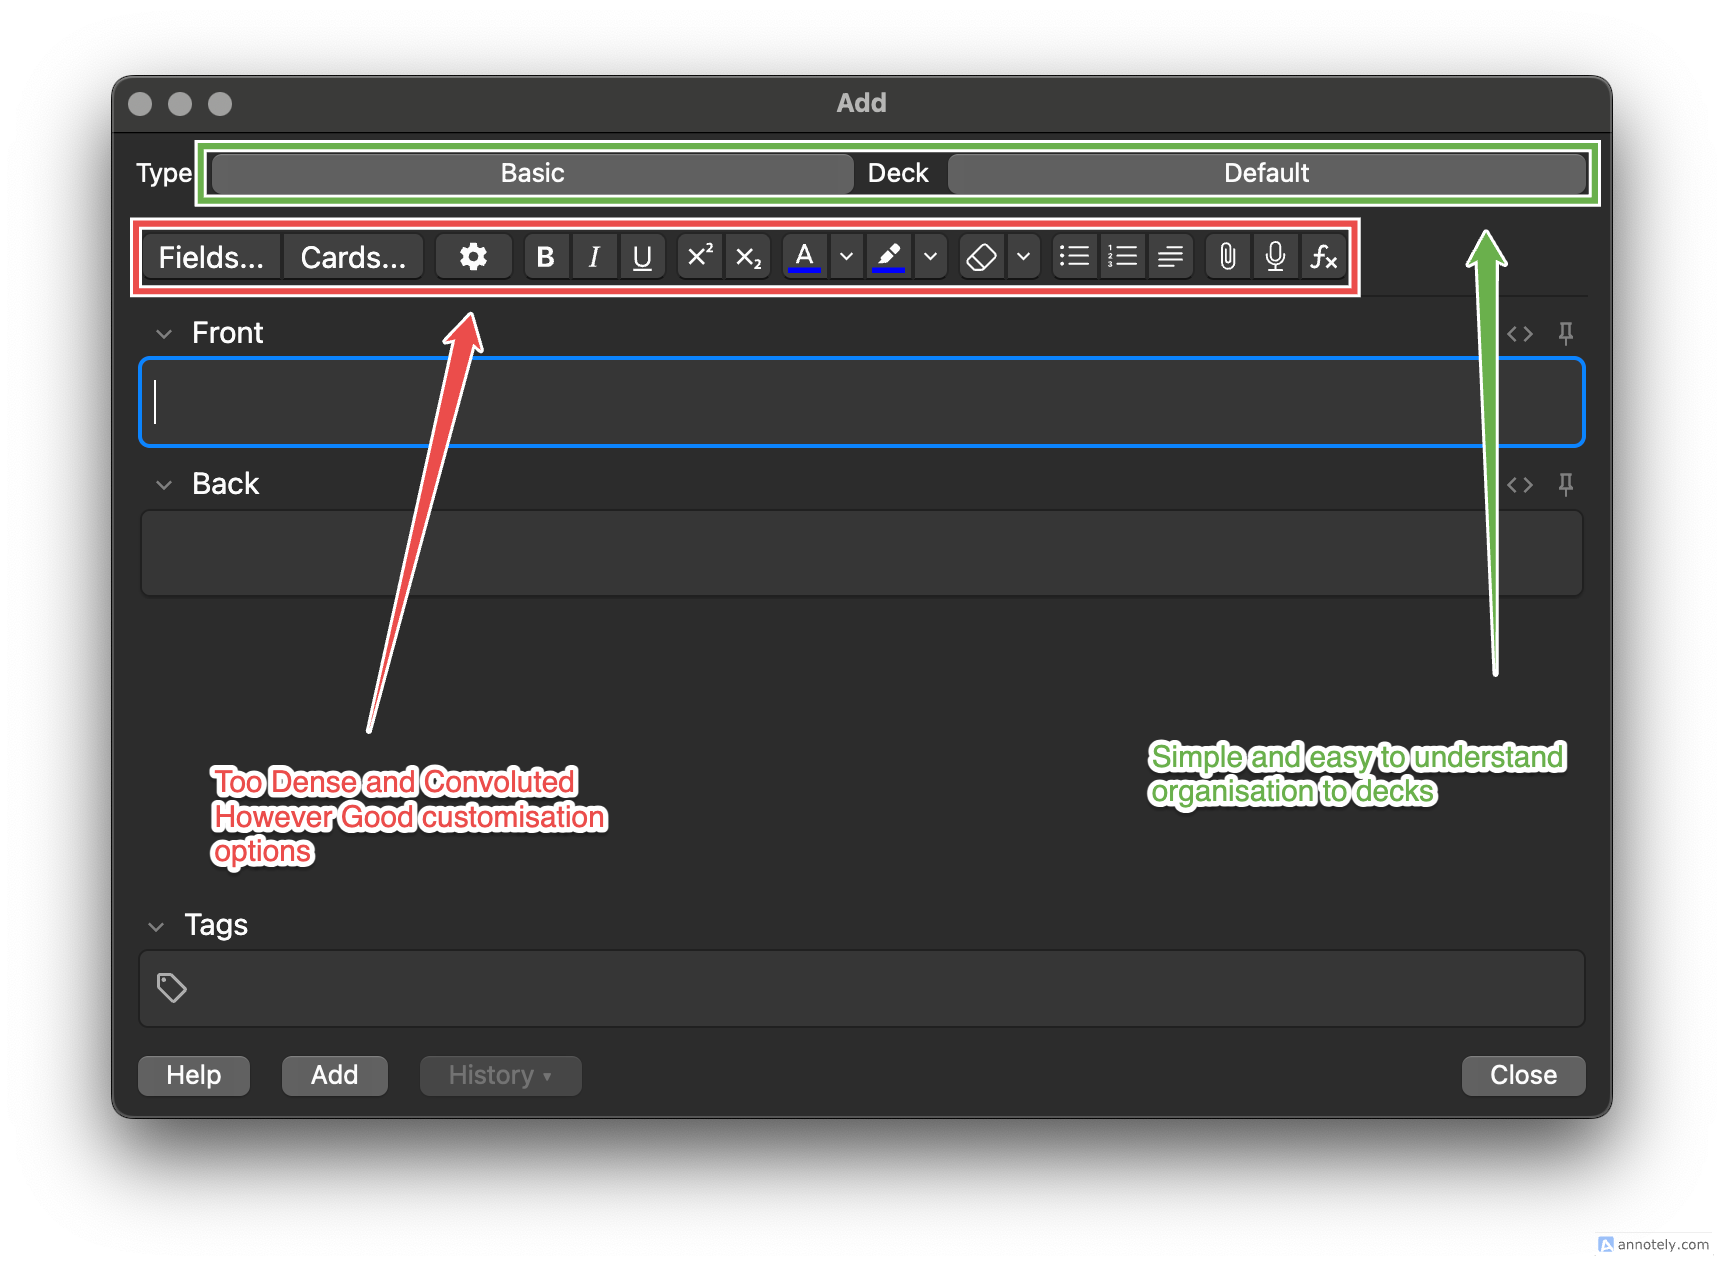
\includegraphics[width=0.7\linewidth]{../Screenshots/AnkiFlashcard.png}
    \caption{Anki Flashcard Menu — interface for creating and editing flashcards}
    \label{fig:anki-flashcard-menu}
\end{figure}

Table~\ref{tab:ankistrengths} summarises the key strengths of Anki, including its core spaced repetition algorithm.

% No \newpage here — let LaTeX figure it out!

	
\begin{ThreePartTable}
\begin{TableNotes}
\footnotesize
\item[*] Planned features are subject to development changes.
\end{TableNotes}
\begin{longtable}{|p{3.5cm}|>{\raggedright\arraybackslash}p{5.5cm}|>{\raggedright\arraybackslash}p{5.5cm}|}
\caption{Anki Features to Keep and Adopt in AI Flashcards App}
\label{tab:ankistrengths} \\
\hline
\textbf{Feature} & \textbf{Why I Like It in Anki} & \textbf{How AI Flashcards App Will Use/Improve It} \\
\hline
\endfirsthead

\multicolumn{3}{c}%
{{\tablename\ \thetable{} -- continued from previous page}} \\
\hline
\textbf{Feature} & \textbf{Why I Like It in Anki} & \textbf{How AI Flashcards App Will Use/Improve It} \\
\hline
\endhead

\hline \multicolumn{3}{r}{{Continued on next page}} \\
\endfoot

\hline
\insertTableNotes
\endlastfoot

Proven Spaced Repetition Algorithm & SM2 algorithm is research-backed and effective & Will implement an adaptive algorithm inspired by SM2 with added AI for confidence-based adjustment* \\
\hline
Rich Media Support & Supports images, audio, video for rich flashcards & Will allow embedded audio, images, and AI-generated podcasts for multi-modal learning* \\
\hline
Cross-Platform Availability & Desktop, iOS, Android versions available & Will support native iOS app plus web with offline sync* \\
\hline
Open Source & Transparent and modifiable codebase & Plan to keep open development with community contributions* \\
\hline
Extensive Customisation & Many settings for advanced users & Provide sensible defaults but allow power users to customise* \\
\hline
Large Community & Shared decks and active user base & Plan to enable deck sharing and community content* \\
\hline
Tagging System & Flexible tagging helps organise decks & Implement simple but powerful tagging and filtering* \\
\hline
Add-ons Ecosystem & Enables powerful third-party extensions & Offer API/plugins to extend app functionality* \\
\hline
Keyboard Shortcuts & Efficient navigation and study flow & Design intuitive shortcuts for faster use* \\
\hline
Statistics Tracking & Basic review stats help monitor progress & Provide enhanced, interactive analytics dashboards* \\
\hline
Support for Multiple Card Types & Basic, cloze deletion, reversed cards & Support popular card types and AI-generated question variations* \\
\hline
Syncing via AnkiWeb & Seamless cross-device sync & Use secure cloud syncing for real-time updates* \\
\hline
Mobile Review Experience & Optimised for small screens & Design minimalistic and effective mobile UI* \\
\hline
Scheduling Flexibility & Adjust intervals manually & Allow users to tweak schedules as needed* \\
\hline
Backup and Export Options & Easy data export for backup & Provide simple backup and export/import features* \\
\hline
Support for LaTeX & Good for math/CS notation & Support LaTeX rendering for technical content* \\
\hline
Tag Hierarchies & Organise decks and cards in nested tags & Plan hierarchical tagging system for better organisation* \\
\hline
Multi-Language Support & Supports cards in any language & Support multilingual flashcards and interface* \\
\hline
Offline Access & Study without internet connection & Full offline functionality with sync on reconnect* \\
\hline
\end{longtable}
\end{ThreePartTable}

\vspace{2em}

\begin{ThreePartTable}
\begin{TableNotes}
\footnotesize
\item[*] Planned features are subject to development changes.
\end{TableNotes}
\begin{longtable}{|p{3.5cm}|>{\raggedright\arraybackslash}p{5.5cm}|>{\raggedright\arraybackslash}p{5.5cm}|}
\caption{Anki Features to Improve and AI Flashcards App Improvement Plans}
\label{tab:anki-features-improve} \\
\hline
\textbf{Feature to Improve} & \textbf{Issue with Anki} & \textbf{Improvement Plan} \\
\hline
\endfirsthead

\multicolumn{3}{c}%
{{\tablename\ \thetable{} -- continued from previous page}} \\
\hline
\textbf{Feature to Improve} & \textbf{Issue with Anki} & \textbf{Improvement Plan} \\
\hline
\endhead

\hline \multicolumn{3}{r}{{Continued on next page}} \\
\endfoot

\hline
\insertTableNotes
\endlastfoot

Steep Learning Curve & Complex UI and manual setup can overwhelm beginners & Simple UI with onboarding tutorials and minimal setup* \\
\hline
Manual Card Creation & Time-consuming and error-prone & Automate flashcard creation using NLP and AI* \\
\hline
Complex Deck Organisation & Nested decks may confuse new users & Start with simple tagging, add hierarchy later* \\
\hline
Lack of Integrated Audio Revision & No built-in audio summaries & Include AI-generated podcasts and TTS* \\
\hline
Limited Built-in Analytics & Requires add-ons for detailed stats & Integrated progress dashboards with insights* \\
\hline
Inconsistent Cross-device Sync & Sync sometimes unreliable & Use cloud backend for real-time sync* \\
\hline
No Built-in Study Guidance & Relies on user self-management & Adaptive spaced repetition driven by confidence* \\
\hline
Overwhelming Customisability & Too many options can confuse users & Sensible defaults with optional advanced settings* \\
\end{longtable}
\end{ThreePartTable}

\vspace{1em}

\textbf{Justification:} 

While Anki’s core features like its spaced repetition algorithm and customisability are industry standards, its complexity and reliance on manual inputs deter many learners. The AI Flashcards App will automate card creation, simplify user experience, and enhance engagement with AI-driven audio and analytics, making effective revision more accessible to a broader audience.

\subsubsection{\underline{Quizlet}}
\begin{figure}[H]
    \centering
    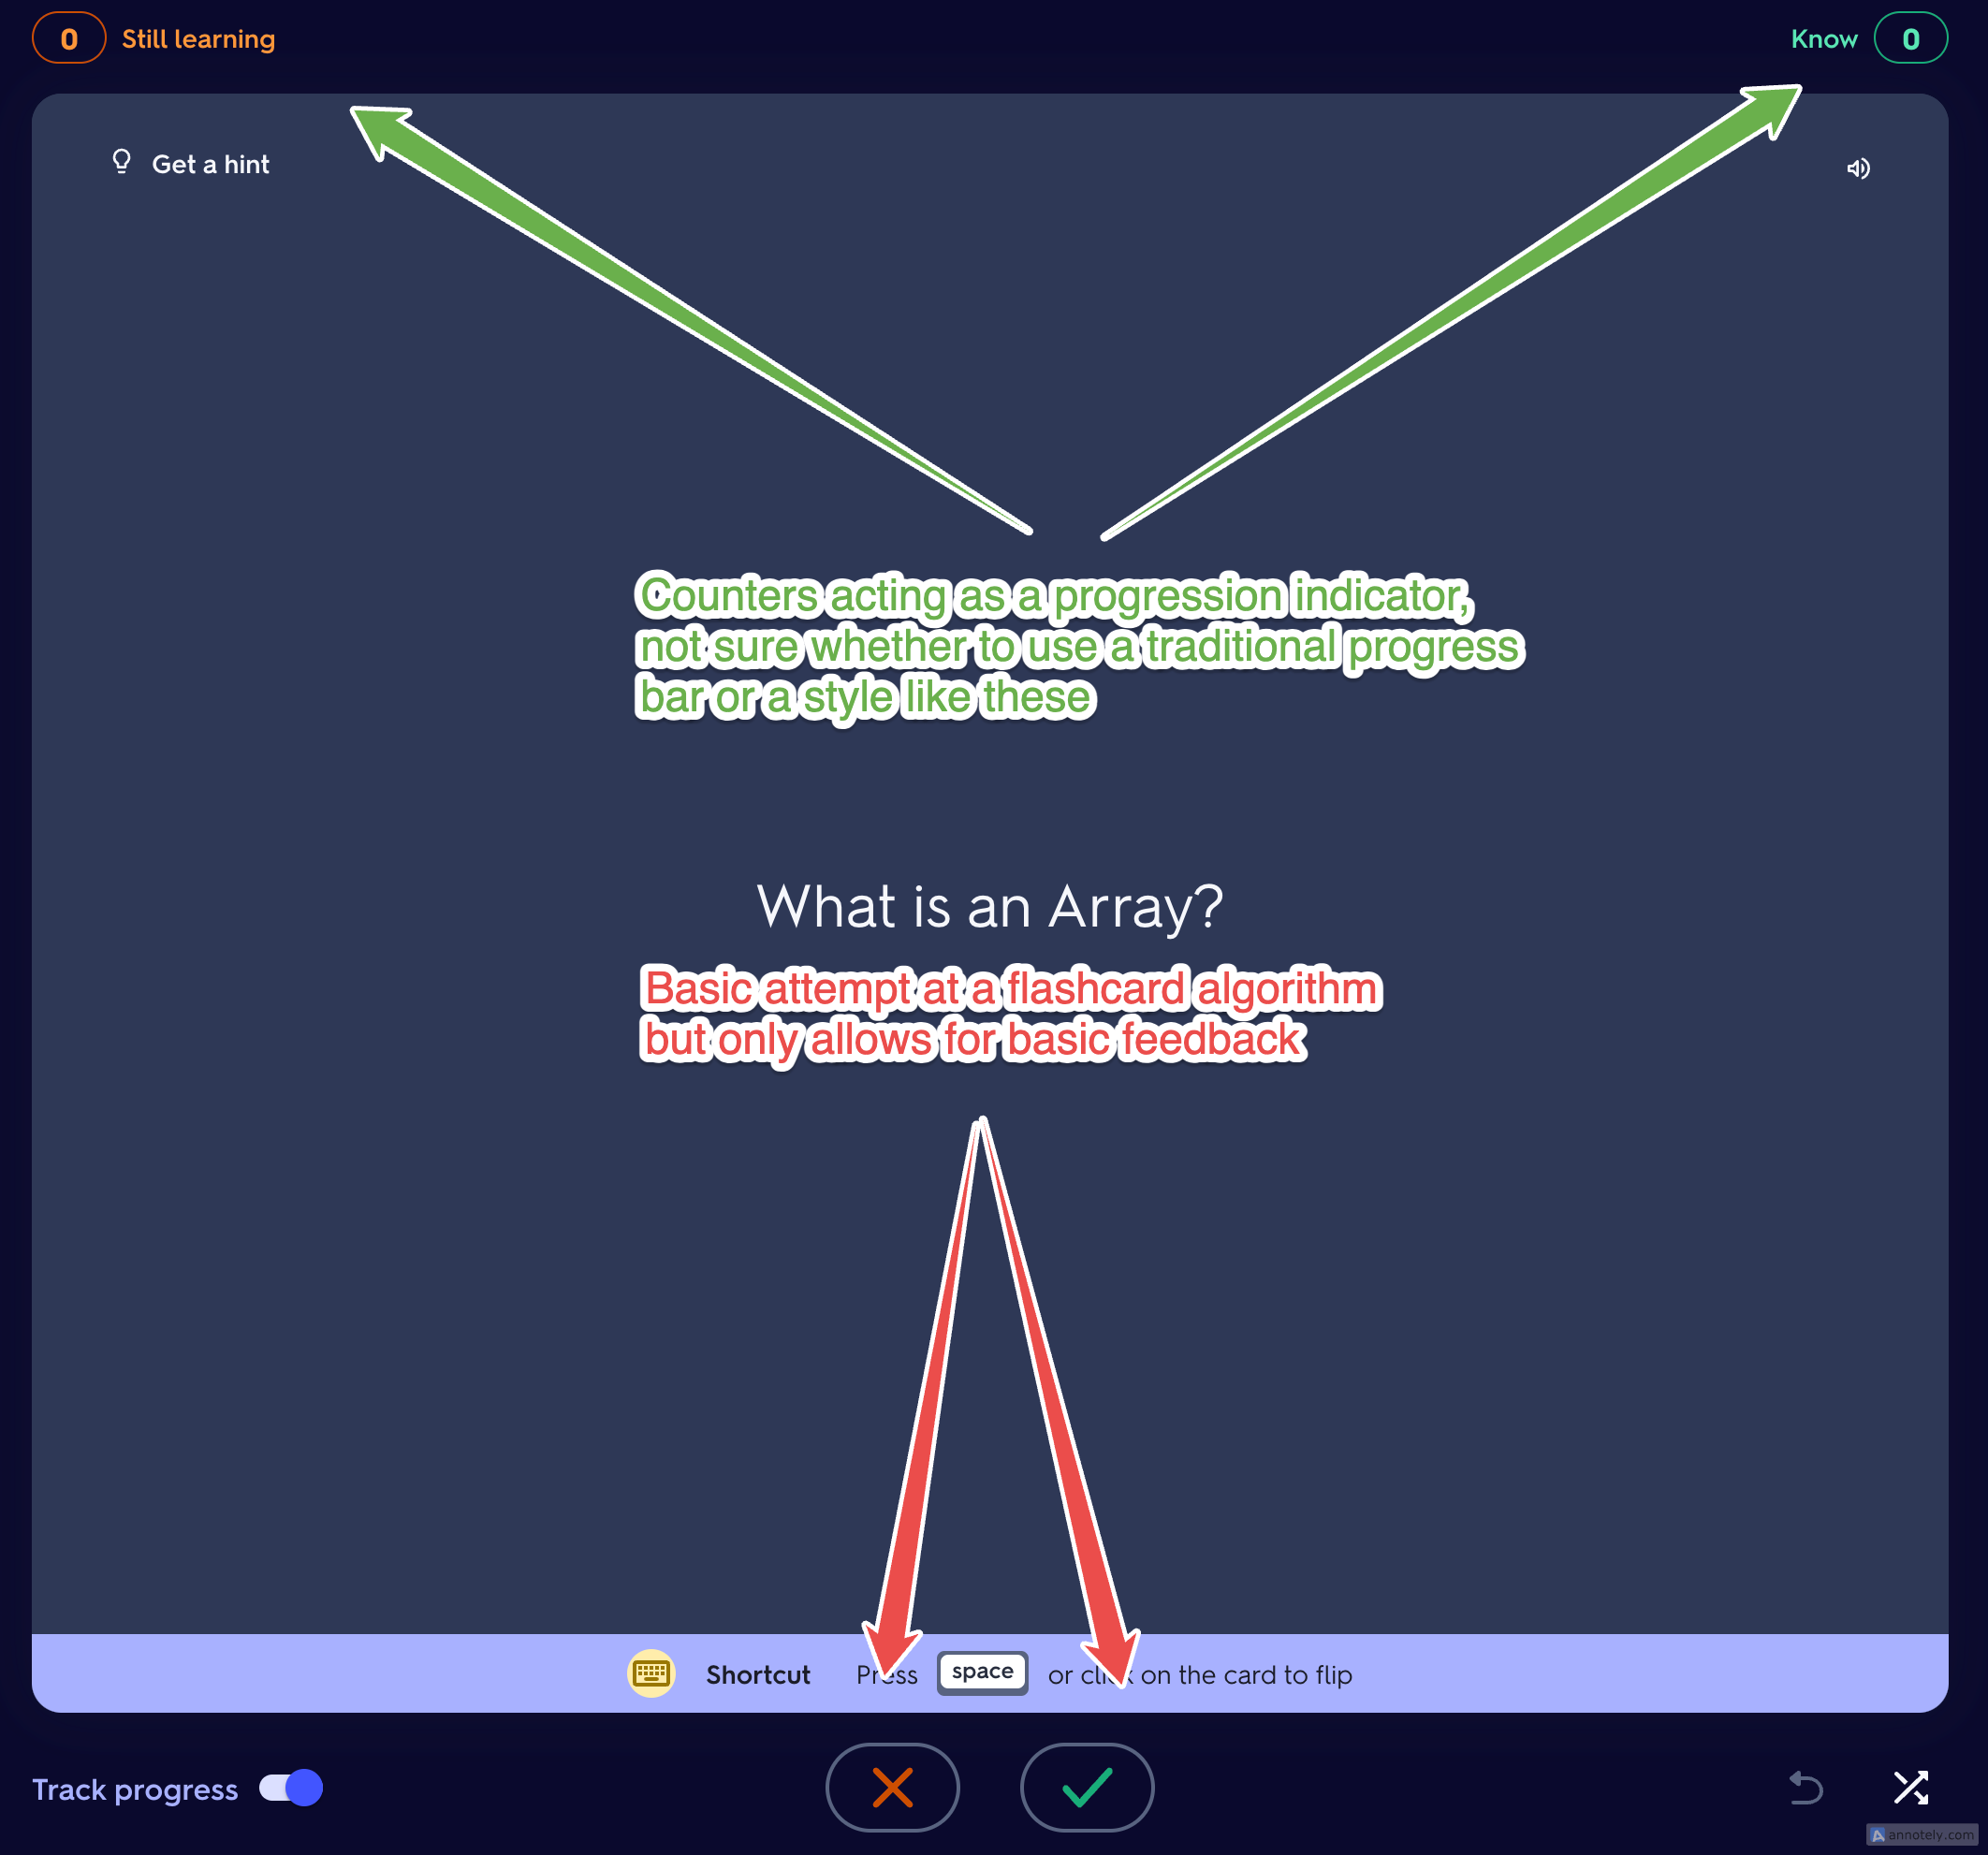
\includegraphics[width=0.7\linewidth]{../Screenshots/QuizletSM2.png}
    \caption{Quizlet Flashcard Revision Menu with Feedback Buttons}
    \label{fig:quizlet-flashcard-menu}
\end{figure}

Quizlet is one of the most widely used flashcard platforms globally, especially popular among school and college students for its simple, user-friendly interface and diverse study modes. Unlike Anki, Quizlet places more emphasis on accessibility and ease of use rather than advanced algorithmic learning techniques. It offers a variety of study activities including flashcards, matching games, multiple-choice tests, and practice quizzes, aiming to engage users through interactive and varied revision styles.\\

Quizlet’s strength lies in its vast community-driven database of shared flashcard sets across countless subjects, allowing users to quickly find ready-made study materials. Its web-based platform and mobile apps (iOS and Android) provide seamless syncing, enabling students to study anytime and anywhere. The platform’s clean design and gamified features appeal especially to younger learners who prefer straightforward, visually engaging revision tools.\\

While Quizlet lacks a formal spaced repetition algorithm, it does provide basic feedback during study sessions, such as marking items “I know” or “I don’t know,” which introduces a minimal level of adaptive learning. It also supports multimedia integration including images and audio, making it useful for language learning and other subjects requiring auditory or visual memory aids.\\

Quizlet operates on a freemium model, offering a free tier with ads and limited features alongside a paid subscription that unlocks additional study modes, offline access, and ad-free use. This model has made Quizlet accessible to millions, but also a target for users who prefer fully free, ad-free educational tools.\\

\begin{ThreePartTable}
\begin{TableNotes}
\footnotesize
\item[*] Planned features are subject to development changes.
\end{TableNotes}
\begin{longtable}{|>{\raggedright\arraybackslash}p{3cm}|>{\raggedright\arraybackslash}p{5cm}|>{\raggedright\arraybackslash}p{5cm}|}
\caption{Quizlet Current Features} \label{tab:quizletfeatures} \\
\hline
\textbf{Feature} & \textbf{Description} \\
\hline
\endfirsthead

\multicolumn{2}{c}%
{{\tablename\ \thetable{} -- continued from previous page}} \\
\hline
\textbf{Feature} & \textbf{Description} \\
\hline
\endhead

\hline \multicolumn{2}{r}{{Continued on next page}} \\
\endfoot

\hline
\insertTableNotes
\endlastfoot
\hline
Collaboration & Limited collaboration features, mostly public deck sharing & Real-time collaborative deck editing with version control and commenting* \\
\hline
AI-Powered Content Generation & No AI-generated content & Automated generation of flashcards, quizzes, and explanations from notes and textbooks* \\
\hline
Personalised Study Plans & No personalised study scheduling & Dynamic study plans tailored to individual goals, deadlines, and learning pace* \\
\hline
Cross-Device Syncing & Basic sync with some delays & Instant cross-device syncing with conflict resolution and offline support* \\
\hline
Accessibility & Basic accessibility options & Enhanced accessibility features including text-to-speech, dyslexia-friendly fonts, and keyboard navigation* \\
\hline
Multimedia Support & Supports images and audio & Expanded multimedia support with video embedding and interactive elements* \\
\hline
Integration & Minimal third-party integration & Integrates with calendars, note apps, and learning management systems (LMS)* \\
\hline
Community Engagement & Basic public decks & Community-driven challenges, leaderboards, and peer feedback systems* \\
\hline
Security & Standard user data protection & End-to-end encryption for user data and private decks* \\
\hline
Custom Feedback & Limited feedback options & AI-driven personalised feedback and hints during study sessions* \\
\hline
\end{longtable}
\end{ThreePartTable}

\vspace{1cm} % space before next table

% Then your improvements table here



\begin{ThreePartTable}
\begin{TableNotes}
\footnotesize
\item[*] Planned features are subject to development changes.
\end{TableNotes}
\begin{longtable}{|p{3.5cm}|>{\raggedright\arraybackslash}p{5.5cm}|>{\raggedright\arraybackslash}p{5.5cm}|}
\caption{Quizlet Features to Improve and Proposed Enhancements}
\label{tab:quizletimprovements} \\
\hline
\textbf{Feature} & \textbf{Current Quizlet} & \textbf{Improvement in AI Flashcards App} \\
\hline
\endfirsthead

\multicolumn{3}{c}%
{{\tablename\ \thetable{} -- continued from previous page}} \\
\hline
\textbf{Feature} & \textbf{Current Quizlet} & \textbf{Improvement in AI Flashcards App} \\
\hline
\endhead

\hline \multicolumn{3}{r}{{Continued on next page}} \\
\endfoot

\hline
\insertTableNotes
\endlastfoot

Adaptive Learning & No formal spaced repetition or algorithm; feedback is limited to “know” or “don’t know” & Implements advanced adaptive spaced repetition algorithm adjusting intervals based on user confidence and performance* \\
\hline
Customisation & Limited card formatting and customization options & Full support for rich text, images, audio, and AI-generated questions* \\
\hline
Pricing Model & Freemium with ads and paid tiers & Fully free with no ads or paywalls, ensuring open access for all users \\
\hline
Analytics & Basic study statistics, no deep progress tracking & Built-in detailed analytics showing learning progress and weaknesses* \\
\hline
Offline Mode & Only with paid subscription & Free offline support planned to maximise accessibility* \\
\hline
Algorithm Transparency & Limited information about underlying learning algorithms & Open and user-transparent adaptive algorithms designed around cognitive science* \\
\hline
Sharing & Public deck sharing but limited collaboration & Plans for seamless collaborative deck creation and sharing* \\
\hline
Content Creation & Mostly manual input by users & Automated note-to-flashcard conversion using AI and NLP* \\
\hline
Mobile Functionality & Good but feature-limited in free version & Full feature parity planned across platforms with mobile optimisation* \\
\hline
Motivation Features & Basic gamification and feedback & Advanced motivational feedback and AI-driven encouragement planned* \\
\hline

\end{longtable}
\end{ThreePartTable}

\begin{figure}[H]
    \centering
    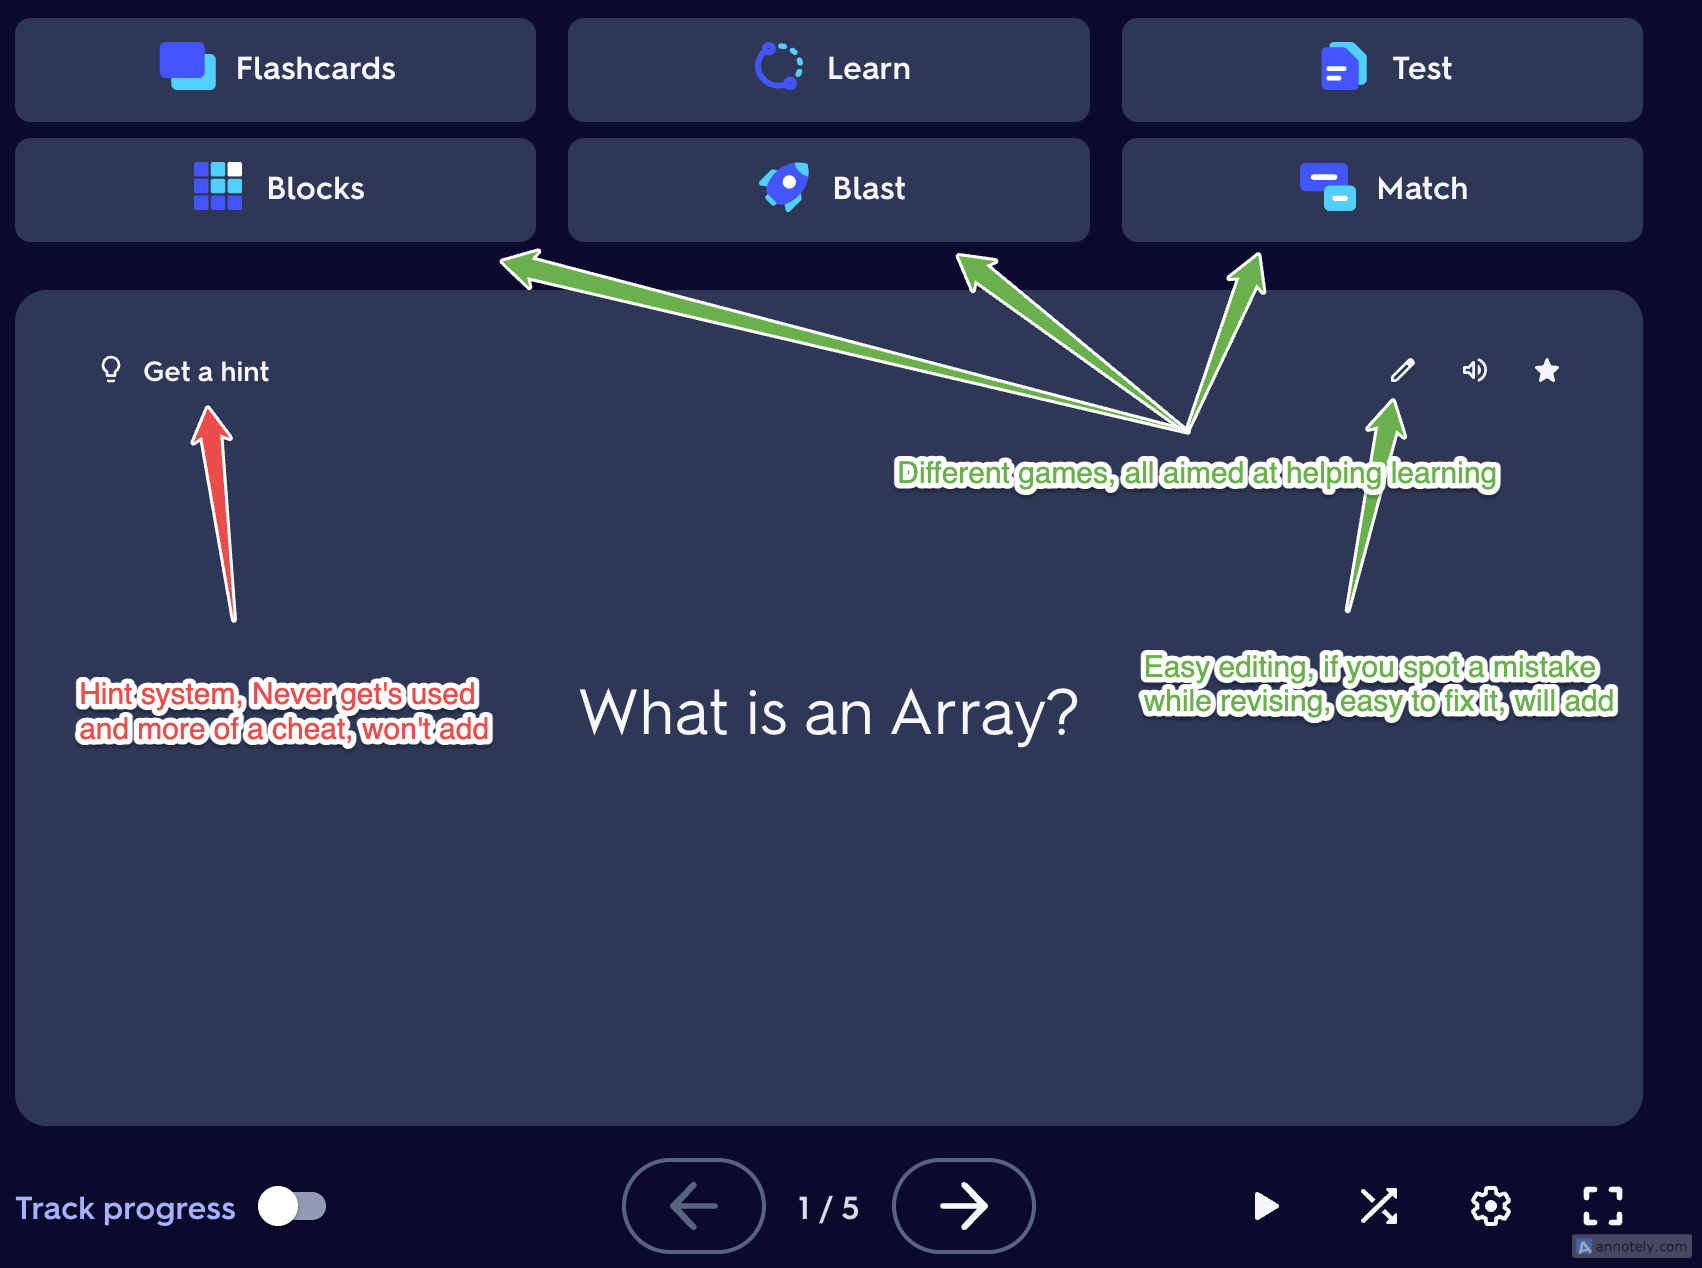
\includegraphics[width=0.5\textwidth]{../Screenshots/QuizletFlashcard.png}
    \caption{Quizlet Flashcard UI}
    \label{fig:quizlethome}
\end{figure}

\subsubsection{\underline{Brainscape}}
Brainscape is an adaptive flashcard app designed to optimise learning through a scientifically backed spaced repetition system. Unlike some other platforms, Brainscape emphasises efficient memorisation by dynamically adjusting the timing of flashcard reviews based on the learner’s confidence ratings. \\
The platform allows users to create their own flashcards or access a vast library of shared content across numerous subjects. Its clean, minimalistic interface is tailored to reduce cognitive load and keep users focused on retention. Brainscape is available on both web and mobile devices, offering seamless syncing to enable study anytime, anywhere. \\

A key feature of Brainscape is its adaptive algorithm which personalises the repetition intervals, making sure that learners review material right before they are likely to forget it. This approach aims to maximise retention while minimising study time, making it particularly popular among students preparing for exams and professionals looking for efficient upskilling. \\

Brainscape operates on a freemium model with a free tier that includes core functionalities, and a premium subscription that unlocks enhanced features such as detailed analytics, expert-created flashcard decks, and offline access. Its focus on cognitive science principles and simplicity has earned it a dedicated user base seeking effective and straightforward study tools. \\

\newpage

\begin{ThreePartTable}
\begin{TableNotes}
\footnotesize
\item[*] Planned features are subject to development changes.
\end{TableNotes}

\begin{longtable}{|p{4cm}|p{5.8cm}|>{\raggedright\arraybackslash}p{5.8cm}|}
\caption{Brainscape Current Features and Usage in AI Flashcards App} \label{tab:brainscapefeatures} \\
\hline
\textbf{Feature} & \textbf{Description} & \textbf{How It’s Used / Justification} \\
\hline
\endfirsthead

\multicolumn{3}{c}%
{{\tablename\ \thetable{} -- continued from previous page}} \\
\hline
\textbf{Feature} & \textbf{Description} & \textbf{How It’s Used / Justification} \\
\hline
\endhead

\hline \multicolumn{3}{r}{{Continued on next page}} \\
\endfoot

\hline
\insertTableNotes
\endlastfoot

Adaptive Spaced Repetition & Dynamically adjusts flashcard review intervals based on user-rated confidence levels. & Core learning logic used to prioritise difficult material and minimise overexposure to mastered content. \\
\hline
User-Generated Content & Users can create and edit their own flashcards and decks manually. & Encourages learner autonomy and allows tailoring of material to individual goals or curricula. \\
\hline
Pre-Made Deck Library & Extensive database of subject-specific flashcard sets available to all users. & Helps users get started quickly or supplement their own decks with expert-vetted material. \\
\hline
Cross-Platform Syncing & Flashcards are synced across devices in real time (web and mobile). & Promotes flexibility and consistency in study routines across different settings. \\
\hline
Minimalist Interface & Clean and distraction-free UI designed for efficiency and focus. & Reduces cognitive load, helping students concentrate on material instead of UI clutter. \\
\hline
Confidence-Based Rating & Users rate their understanding after each flashcard from 1 (low) to 5 (high). & Drives the adaptive algorithm, ensuring the system targets weak areas more frequently. \\
\hline
Premium Subscription & Unlocks extra features including offline access, advanced stats, and expert content. & Monetises the platform but restricts access to helpful features without payment. \\
\hline
Basic Analytics & Tracks study time, confidence history, and subject progress in a simplified dashboard. & Offers limited insight to support performance tracking, but lacks diagnostic depth. \\
\hline
Deck Organisation & Users can group related flashcards into folders and subfolders. & Improves content navigation and management for complex subjects or courses. \\
\hline
Simple Gamification & Offers badges and streak tracking to promote consistent study habits. & Provides light motivational incentives without being overly game-like. \\
\hline
Limited Collaboration & No multi-user deck editing or shared learning sessions. & Restricts cooperative learning, which could be addressed in a future app version. \\
\hline
Text-Only Focus & Lacks support for audio, images, or rich formatting. & Limits effectiveness for visual or auditory learners; an area for clear enhancement. \\
\hline
\end{longtable}
\end{ThreePartTable}

\vspace{1cm}

\begin{ThreePartTable}
\begin{TableNotes}
\footnotesize
\item[*] Planned features are subject to development changes.
\end{TableNotes}

\begin{longtable}{|p{3.5cm}|>{\raggedright\arraybackslash}p{6cm}|>{\raggedright\arraybackslash}p{5.5cm}|}
\caption{Proposed Improvements Over Brainscape Features in AI Flashcards App} \label{tab:brainscapeimprovements} \\
\hline
\textbf{Feature} & \textbf{Current Brainscape} & \textbf{Improvement in AI Flashcards App} \\
\hline
\endfirsthead

\multicolumn{3}{c}%
{{\tablename\ \thetable{} -- continued from previous page}} \\
\hline
\textbf{Feature} & \textbf{Current Brainscape} & \textbf{Improvement in AI Flashcards App} \\
\hline
\endhead

\hline \multicolumn{3}{r}{{Continued on next page}} \\
\endfoot

\hline
\insertTableNotes
\endlastfoot

Adaptive Spaced Repetition & Dynamic review based on confidence ratings & Incorporates AI to adjust intervals considering cognitive load, forgetting curves, and user behaviour for maximised retention* \\
\hline
User-Generated Content & User-created decks & AI-assisted deck creation from notes and textbooks, reducing manual effort* \\
\hline
Pre-Made Deck Library & Large collection of expert and community decks & Crowdsourced and AI-curated decks with quality ratings and personalised recommendations* \\
\hline
Cross-Platform Syncing & Web, iOS, and Android syncing & Real-time syncing with conflict resolution and offline editing support* \\
\hline
Clean Interface & Minimalist, distraction-free & Customisable UI themes and layouts tailored to user preferences* \\
\hline
Confidence-Based Rating & User self-rates knowledge & AI-estimated confidence using interaction data plus user input for improved scheduling* \\
\hline
Premium Subscription & Paid unlocks for analytics and offline & Fully free core features with optional privacy-respecting donations and unlocked analytics* \\
\hline

\end{longtable}
\end{ThreePartTable}

\begin{figure}[H]
  \centering
  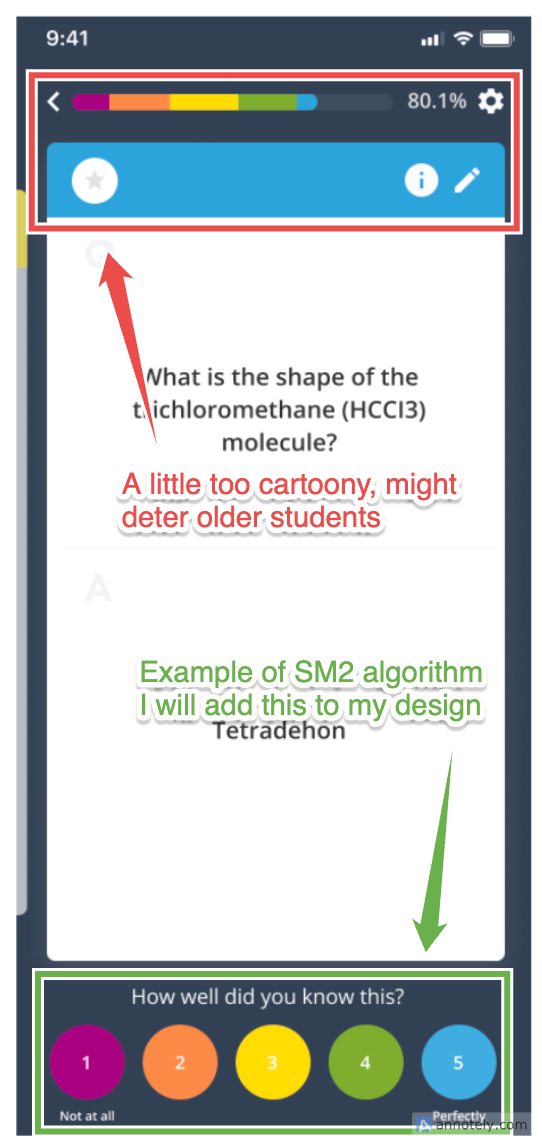
\includegraphics[width=0.2\textwidth]{../Screenshots/BrainscapeFlashcard.png}
  \caption{Brainscape Home Screen}
  \label{fig:brainscapehome} % unique label
\end{figure}

\newpage

\subsection{The SM-2 Algorithm and Mathematical Scheduling}

A fundamental feature of Anki, and the one most directly influencing my own solution, is it's use of the SM-2 spaced repetition algorithm. This algorithm was developed by Piotr Wozniak in 1985 for SuperMemo and is designed to determine optimal review intervals using user feedback on recall difficulty. Spaced repetition, when grounded in algorithms like SM2, improves memory retention through the spacing effect, a psychological phenomenon that shows information is better remembered when exposures are spaced over time. \\

The core idea is to calculate a new interval $I_n$ after each review, based on the user's performance, using a formula influenced by both previous interval and an ease factor. SM2 adjusts this ease factor ($EF$) based on how well the user remembers the item. \\

\medskip

The general logic follows these rules:

\begin{itemize}
  \item If the user grades their recall quality less than 3 (on a scale from 0 to 5), the item is scheduled to be reviewed again soon — usually the next day.
  \item If the grade is 3 or above, a new interval is calculated:
    \begin{align*}
      I_1 &= 1 \\
      I_2 &= 6 \\
      I_n &= I_{n-1} \cdot EF \quad \text{for } n > 2
    \end{align*}
  \item The ease factor is updated as follows:
    \[
    EF' = EF - 0.8 + (0.28 \cdot q) - (0.02 \cdot q^2)
    \]
    where $q$ is the quality of the response (0–5), and $EF$ is constrained to a minimum of 1.3.
\end{itemize}

The exponential nature of the interval calculation allows well-remembered items to be reviewed far less frequently over time, conserving cognitive effort for more difficult items. For instance, if a card is repeatedly recalled successfully with a consistent $EF$ of 2.5, the intervals will expand rapidly: 1 day, 6 days, 15 days, 37 days, 92 days, and so on. This aligns with human forgetting curves, where memory retention drops off sharply at first, but then levels off. \\

From a computational standpoint, this algorithm is a perfect example of a lightweight yet effective method for intelligent scheduling. It uses basic arithmetic and quadratic expressions to adapt to the user's performance without requiring complex machine learning techniques, making it highly suitable for low-power or offline devices like a smartphone. \\

\medskip

I intend to implement a simplified or modified version of the SM-2 algorithm in my project. The scheduling function will track user performance on each flashcard and update review intervals using a similar exponential model. This will allow my app to tailor repetition to individual users in a mathematically sound way. \\

\medskip

\noindent This feature is crucial to the effectiveness of spaced repetition tools and is a key component I will adopt and adapt for my own app.\footnote{SM-2 was first introduced by Piotr Wozniak as part of the SuperMemo project. See a detailed breakdown here: \href{https://help.remnote.com/en/articles/6026144-the-anki-sm-2-spaced-repetition-algorithm}{RemNote SM-2 Guide}.}

\newpage

\subsection{Essential Features of the Proposed Solution}
\begin{ThreePartTable}
\begin{TableNotes}
\footnotesize
\item[*] Feature implementation may vary slightly depending on development constraints.
\end{TableNotes}

\begin{longtable}{|>{\raggedright\arraybackslash}p{3.5cm}|>{\raggedright\arraybackslash}p{5.5cm}|>{\raggedright\arraybackslash}p{5.5cm}|}
\caption{Essential Features of the Proposed Solution} \label{tab:essentialfeatures} \\
\hline
\textbf{Feature} & \textbf{Justification} & \textbf{How It Will Be Used} \\
\hline
\endfirsthead

\multicolumn{3}{c}%
{{\tablename\ \thetable{} -- continued from previous page}} \\
\hline
\textbf{Feature} & \textbf{Justification} & \textbf{How It Will Be Used} \\
\hline
\endhead

\hline \multicolumn{3}{r}{{Continued on next page}} \\
\endfoot

\hline
\insertTableNotes
\endlastfoot

Automated Flashcard Generation & Reduces manual work and speeds up revision preparation, making it more accessible and less time-consuming & Notes (PDF or text) will be scanned and converted into flashcards using NLP to extract key points, definitions, and questions \\
\hline

Spaced Repetition Algorithm & Supports efficient memorisation by using proven cognitive science techniques & Flashcard intervals will adapt based on user confidence and performance, enhancing long-term retention \\
\hline

Custom Deck Management & Allows personalisation and structured revision & Users can create and categorise decks by subject, topic, or difficulty level; changes sync across sessions \\
\hline

AI Feedback and Motivation & Keeps users engaged and encourages continued use of the app & System provides encouragement, reminders, and tailored progress feedback after each study session \\
\hline

Multi-Modal Learning Support & Supports a wider range of learning styles and increases accessibility & Flashcards can be read aloud using text-to-speech or summarised in short AI-generated podcasts \\
\hline

Cross-Platform Accessibility & Ensures usability across different environments and devices & Both desktop and mobile versions will offer the same core features and sync data between platforms \\
\hline

Simple, Intuitive UI/UX & Prevents cognitive overload and supports a better user experience & Interface designed with clean visuals, minimal distractions, and easy navigation for students \\
\hline

Data-Driven Progress Analytics & Helps users identify weak areas and track improvements over time & Provides visual feedback on accuracy, study time, and topics requiring further revision \\
\hline

\end{longtable}
\end{ThreePartTable}

\newpage

\subsection{Limitations of the Proposed Solution}

Despite its innovative and educationally valuable features, Delphi has a number of limitations that reflect both practical development constraints and technical boundaries:

\begin{itemize}
    \item \textbf{Natural Language Processing (NLP) Reliability:} While NLP techniques enable automatic flashcard generation from user notes, these models can struggle with handwritten input, poorly structured text, or domain-specific terminology. Misinterpretations may result in irrelevant or inaccurate questions. Furthermore, without advanced fine-tuning, the generated content may lack pedagogical depth or consistency with user expectations.
    
    \item \textbf{Generalised AI Models Without User Personalisation:} The AI used for flashcard and quiz generation is based on general-purpose large language models (LLMs) and lacks deep user personalisation. It does not adapt to individual user performance over time, learning style preferences, or cognitive strengths/weaknesses. Fully adaptive AI would require complex reinforcement learning pipelines and continuous user data collection, which are outside the scope of this project.
    
    \item \textbf{AI Feedback May Lack Pedagogical Rigor:} Although the system aims to offer automated encouragement and performance feedback, AI-generated feedback may sometimes be vague, overly generic, or misleading. Without expert-curated intervention, this could negatively impact user confidence or learning outcomes in some cases.
    
    \item \textbf{Computational Constraints and Offline Limitations:} While AI features such as flashcard generation, summarisation, and feedback significantly enhance the app’s learning potential, they introduce considerable computational demands. Running these models locally---especially on mobile devices---is largely impractical due to limited processing power, memory, and battery capacity. As a result, during development, AI inference may need to be offloaded to a more powerful personal computer or external server. This introduces dependency on internet connectivity and backend infrastructure, reducing offline availability. Furthermore, compressing models for on-device deployment can reduce their accuracy and effectiveness. Full offline parity would require bundling large language models into the app, significantly increasing its size, reducing device compatibility, and introducing additional privacy and update challenges.
    
    \item \textbf{Lack of Secure User Accounts:} The current version of the solution does not include user account management, login, or profile-based data storage. This limits long-term tracking of user progress, cross-device syncing, and personalised content retrieval. While it reduces complexity and protects user anonymity, it also restricts the app’s potential for growth and community features.
    
    \item \textbf{Device and Platform Limitations:} The app is designed primarily for iOS using Swift, and does not currently support Android or web platforms. Additionally, older devices may struggle with rendering or processing-intensive tasks such as text-to-speech or AI-generated flashcards.
    
    \item \textbf{Limited Gamification and Motivation Systems:} Although motivational AI feedback is planned, more advanced features like leaderboards, community challenges, or reward systems are not included in this release. This could reduce long-term user engagement compared to platforms with stronger gamified ecosystems.
    
    \item \textbf{Data Privacy Considerations:} While no sensitive personal data is stored, the app will still process educational material and user-generated notes. Without full end-to-end encryption and local AI inference, there remains a minor risk of data exposure when using external APIs or cloud services. This is especially relevant in school environments or for underage users.
\end{itemize}
\subsection{Requirements}

\subsubsection*{Software Requirements}
\begin{itemize}
  \item iPhone with iOS 17 or later
\end{itemize}

\subsubsection*{Hardware Requirements}
\begin{itemize}
  \item recent iPhone or iPad (iPhone 8+ minimum, 11+ recommended)
\end{itemize}

\subsection{Success Criteria}

\documentclass{article}
\usepackage{tabularx}
\usepackage{booktabs}
\usepackage[utf8]{inputenc}
\usepackage[T1]{fontenc}

\begin{document}

\begin{table}[ht]
\centering
\caption{Success Criteria for Delphi}
\begin{tabularx}{\textwidth}{@{} p{0.15\textwidth} p{0.35\textwidth} X @{}}
\toprule
\textbf{Criterion ID} & \textbf{Success Criterion} & \textbf{Justification} \\
\midrule
SC1 & Users must be able to create, edit, and delete custom flashcards. & Essential core functionality for user-generated content. Measured by confirming each operation works from the UI. \\
SC2 & The system must implement spaced repetition based on recall history. & Supports memory retention through proven pedagogical methods. Verified via scheduled card review logic. \\
SC3 & Users must classify their recall as ``Known'', ``Unsure'', or ``Don’t Know'' per flashcard. & Allows the system to personalise revision. Measured by ensuring user input affects scheduling. \\
SC4 & A functional onboarding screen must display on first launch and be accessible later. & Assists new users in understanding how to use the app. Checked via first-run and help-button testing. \\
SC5 & The app must save user data and flashcards locally, persisting between sessions. & Crucial for offline usability and session continuity. Verified through local data inspection and app restarts. \\
SC6 & The app must be fully usable offline with no crashes or data loss. & Ensures reliability in various real-world use cases (e.g. school WiFi blocks). Verified by disabling network and testing full flow. \\
SC7 & The app must load in under 2 seconds on a Raspberry Pi 4B. & Demonstrates responsiveness on low-power hardware. Measured using a stopwatch from launch to usability. \\
SC8 & Each flashcard must support both text and image content. & Enhances engagement and caters to different learning styles. Verified through media attachment and rendering. \\
SC9 & Cards must be taggable with categories and filterable by tag. & Enables focused revision sessions. Measured by confirming tags can be added, removed, and used to filter. \\

\bottomrule
\end{tabularx}
\end{table}

\end{document}

\section{Design}

\subsection{Breaking Down the Problem into Smaller Computational Subproblems}

The core problem — helping students revise effectively by converting notes into intelligent flashcards and delivering adaptive learning — is too broad to solve as a single monolithic task. Therefore, it must be systematically decomposed into smaller, manageable subproblems, each suitable for computational methods.

\subsubsection*{1. Input Processing: Accepting and Understanding Study Materials}

\begin{itemize}
    \item \textbf{Problem:} Students have diverse note formats — typed summaries, PDFs, images, or even audio. The app must accept these inputs and prepare them for further processing.
    \item \textbf{Justification:} Automating the conversion of study materials into flashcards requires robust input parsing. Initially focusing on typed text and PDFs simplifies the scope while covering the most common use cases.
    \item \textbf{Computational approach:} Use text extraction libraries to convert PDFs into plain text, and design a parser that can segment the text into logical chunks (e.g., paragraphs or headings) that can later be transformed into flashcards.
\end{itemize}

\subsubsection*{2. Content Extraction and Flashcard Generation}

\begin{itemize}
    \item \textbf{Problem:} Raw text must be analysed and broken down into meaningful questions and answers suitable for flashcards.
    \item \textbf{Justification:} Manual flashcard creation is time-consuming and inconsistent. Automating this step saves time and ensures a more objective, systematic question generation.
    \item \textbf{Computational approach:} Implement lightweight Natural Language Processing (NLP) techniques to identify key concepts, keywords, and definitions within the notes. This includes:
    \begin{itemize}
        \item Keyword extraction (e.g., TF-IDF or basic term frequency analysis)
        \item Named entity recognition for key terms
        \item Sentence simplification or summarisation to create clear question-answer pairs
        \item Basic template generation (e.g., “What is X?”, “Explain Y”)
    \end{itemize}
\end{itemize}

\subsubsection*{3. Data Storage and Organisation}

\begin{itemize}
    \item \textbf{Problem:} Generated flashcards must be stored efficiently and organised into decks, accessible for review.
    \item \textbf{Justification:} Students need to categorise and retrieve flashcards easily to study specific subjects or topics.
    \item \textbf{Computational approach:} Design a data structure (such as a database or persistent JSON files) to store flashcard objects with metadata (deck name, tags, difficulty). Allow CRUD (Create, Read, Update, Delete) operations on cards.
\end{itemize}

\subsubsection*{4. Adaptive Learning and Spaced Repetition}

\begin{itemize}
    \item \textbf{Problem:} To maximise retention, the app must prioritise cards for review based on user performance and proven cognitive science principles.
    \item \textbf{Justification:} Spaced repetition is a well-established technique shown to improve memory retention by optimising review intervals.
    \item \textbf{Computational approach:} Implement a variation of the SM-2 spaced repetition algorithm or a confidence-based ranking system to schedule flashcard reviews dynamically based on user feedback and scores.
\end{itemize}

\subsubsection*{5. User Interaction and Feedback}

\begin{itemize}
    \item \textbf{Problem:} The app should provide intuitive navigation, editable flashcards, and visual feedback to support engagement and self-assessment.
    \item \textbf{Justification:} Usability is crucial to encourage consistent use, while allowing edits ensures users can fix inaccuracies from automated generation.
    \item \textbf{Computational approach:} Design a responsive UI with editable fields and simple controls for marking cards as ‘easy,’ ‘hard,’ or ‘again.’ Provide progress tracking and statistics.
\end{itemize}

\subsubsection*{6. Multimedia and Audio Integration}

\begin{itemize}
    \item \textbf{Problem:} Some learners benefit from multimodal revision — images, audio summaries, or mini podcasts.
    \item \textbf{Justification:} Providing alternative input and revision modes caters to different learning styles, increasing accessibility and engagement.
    \item \textbf{Computational approach:} Integrate text-to-speech (TTS) features to generate audio flashcards or podcast-style summaries automatically, enhancing learning on the go.
\end{itemize}


Each of these subproblems has been considered separately during development to ensure modularity, ease of testing, and maintainability.

\subsection{Structure of the Solution}

The app will be structured as a modular system, comprising the following components:

\begin{itemize}
  \item \textbf{Frontend (iOS app in Swift):} Handles user interface, navigation, flashcard display, and interaction.
  \item \textbf{Backend AI/NLP Module (Python):} Processes notes to generate flashcards using NLP techniques.
  \item \textbf{Data Layer:} Manages local storage of flashcards, user settings, and progress tracking.
  \item \textbf{Audio Engine:} Converts flashcards into audio format using text-to-speech APIs.
  \item \textbf{Spaced Repetition Scheduler:} Uses an adaptation of the SM-2 algorithm to schedule flashcard reviews.
\end{itemize}

The following diagram illustrates the interactions between components:

\subsection{Algorithm Design and Justification}

\subsubsection*{Flashcard Generation Algorithm}

Using NLP techniques such as keyword extraction and sentence parsing, the backend processes uploaded notes to identify important facts and concepts. These are converted into flashcard pairs via rule-based templates and heuristics.

This approach balances simplicity with effectiveness, avoiding overly complex machine learning models that exceed the project scope and resources. It ensures flashcards remain relevant and understandable.

\subsubsection*{Spaced Repetition Algorithm}

The app uses a simplified adaptation of the SM-2 algorithm, which dynamically adjusts intervals between flashcard reviews based on user performance scores (e.g., “Easy”, “Hard”, “Forgot”).

This algorithm is proven to optimise long-term retention by spacing reviews at increasing intervals, tailored to the user’s memory strength per card.

\subsection{Usability Features and Justification}

Key usability features include:

\begin{itemize}
  \item \textbf{Simple, Clean UI:} Designed for minimal cognitive load, enabling quick navigation and effortless review sessions.
  \item \textbf{Offline Mode:} Allows uninterrupted access to flashcards without internet, catering to on-the-go revision.
  \item \textbf{Editable Flashcards:} Users can modify generated cards to correct errors or personalise content, improving learning effectiveness.
  \item \textbf{Organisable Decks:} Enables categorisation by subject or topic for targeted revision.
  \item \textbf{Audio Revision:} Supports diverse learning styles by providing an auditory revision option.
  \item \textbf{Notifications and Streaks:} Encourages consistent use through reminders and progress tracking, increasing engagement.
\end{itemize}

These features align with the needs of the primary stakeholder and reflect best practices in educational app design.

\newpage

\subsection{Key Variables, Data Structures, and Classes}

\begin{table}[h]
\centering
\begin{tabular}{|>{\raggedright\arraybackslash}p{0.2\linewidth}|>{\raggedright\arraybackslash}p{0.35\linewidth}|>{\raggedright\arraybackslash}p{0.2\linewidth}|>{\raggedright\arraybackslash}p{0.2\linewidth}|}
\hline
\textbf{Identifier} & \textbf{Description} & \textbf{Data Type} & \textbf{Validation (if any)} \\
\hline
\texttt{flashcardList} & Stores all flashcards created by the user. & List of dictionaries & Valid JSON structure \\
\hline
\texttt{question} & The question or front side of a flashcard. & String & Non-empty, under 200 characters \\
\hline
\texttt{answer} & The answer or back side of a flashcard. & String & Non-empty, under 300 characters \\
\hline
\texttt{reviewInterval} & Days until the card is shown again (spaced repetition). & Must be \(\geq 1\) \\
\hline
\texttt{lastReviewed} & Date the card was last reviewed. & Date (ISO 8601) & Valid date format (e.g. \texttt{2025-06-23}) \\
\hline
\texttt{userSettings} & Stores theme, AI toggle, etc. & Dictionary & Must include defaults if unset \\
\hline
\texttt{aiEnabled} & Determines whether AI suggestions are on. & Boolean & True or False only \\
\hline
\end{tabular}
\caption{Key Variables Used in the Application}
\label{tab:keyvariables}
\end{table}

\subsection{Test Data Identification and Justification}

\textbf{During development, the following test data will be used:}

\begin{itemize}
  \item \textbf{Sample PDFs:} Notes from subjects such as Computer Science and Economics, representing typical input content.
  \item \textbf{Edge Case Text Files:} Minimal content, empty files, or corrupted PDFs to test robustness.
  \item \textbf{User Interaction Scenarios:} Predefined flashcard decks with varying numbers of cards to test navigation, editing, and spaced repetition.
  \item \textbf{Performance Data:} Simulated user scores (“Easy”, “Medium”, “Hard”) to verify spaced repetition scheduling.
\end{itemize}

\subsection{Post-Development Data and Evaluation}

Post-deployment, anonymised user data on revision patterns, flashcard usage frequency, and retention outcomes will be collected (with consent) to evaluate effectiveness and guide future improvements.

This data includes:

\begin{itemize}
  \item Flashcard review logs (timestamps and user ratings)
  \item Deck usage statistics
  \item Audio revision session counts
  \item User feedback from in-app surveys
\end{itemize}
\end{document}
